\section{Graphical Design}
When you dive into the ocean of possibilities that is design, there are many factors to be considered. What color palette should you choose? And which fonts goes best together. How do you find your way through mixing the right colors and fonts? And how does this affect the way your design is being perceived? 

Two of the things people often complaint about in applications is a confusing interface design and poor navigation. \cite{Pattern} This can be prevented by using design patterns. 
First, let's look at navigation. There are two ways to make navigating through an app easier. Persistent and transient. Persistent navigation is your list menus and your tab menus or menu structures if you will. Transient navigation has to be revealed through a tab action or the likes.\cite{Pattern}
Does the user need to see the menu at all times? If not, you can use an off-canvas solution like the side bar. 
It has become more and more popular to use off canvas methods. \cite{Pattern} This helps the app hold more information but without being confusing e.g. If all your information has to go on one page. 

You don't want to put too much text into one page or have a simple form take up several pages. A sign in for example should only be one page. A way to not get an over lapping look is by using vertical labels instead of horizontal. \cite{Pattern} Or you could have the horizontal labels where the text disappears as soon as the user starts typing, but you risk that the user forgets what they should fill in.\cite{Pattern} 
Some apps, like Instagram, shows the "sign in" and "sign up" option all the way through the tutorial. This also insures that the user do not have to go through a whole tutorial if they don’t need it. 

Keeping these patterns in mind there are still many things to consider. 
First of all, remember the size of the screen that you are designing for. Avoid using big scaled photos and put to much information at one page. This will make it look cluttered and make it less intuitive. \cite{Graphic}
In short, make everything as clean and simple as possible. 

\subsubsection{Colors}

Colours are not just colours when you are designing a brand, an app or a website. Colours are perceived in various ways and is a big part of how your design is coming  across to the user. \cite{Colormeaning}
But first things first, let's have a look at what colours consists of.

There are to primary colours. Additive and subtractive. Additive is used on screens as it gives away light and subtractive is used for e.g. book covers as it reflects light. \cite{Colour}
These are also known as RGB(Red, blue and green) and CMYK(Cyan, magenta and yellow).
In additive colours white is colours mixed together where black is the absence of colour. In subtractive white is the absence of colour and black all the colours mixed together. 
Since subtractive colour do not fully absorb light a fourth element has been added, hence the K in CMYK. K stand for 'key' which essentially is black.\cite{Colour}

The colour wheel can helps us see which colours are complimentary, adjacent and triadic. 
\begin{figure}[H]
\centering
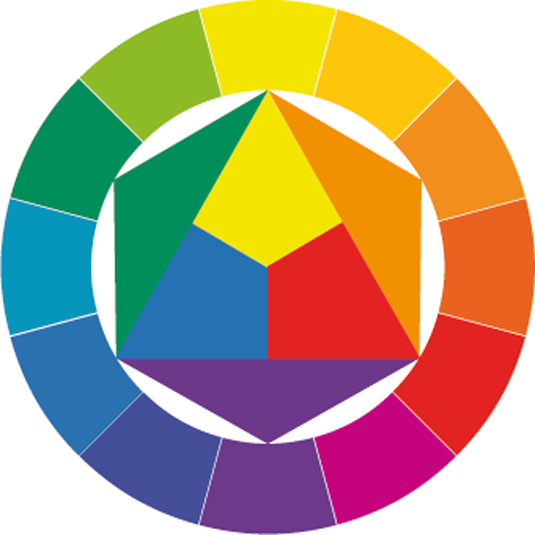
\includegraphics[scale=0.25]{wheel.png}
\caption{The colour wheel. \cite{Colour}}
\end{figure}

Colours are defined by hue, saturation and brightness. 
Using a colour gamut you can see all the different shades available. As you will discover, the RGB is much more limited than CMYK. This is because there is a limit to how much a screen is able to show. 

It is important to remember that when choosing the colour palette for a design that how we perceive colour is very different. Also, colours can change according to what you put it next to. Yellow might look different next to grey than it will next to purple for instances. \cite{Colour}

When it comes to color psychology the truth is, it is too dependent on personal experience. There is no one right answer to which color falls into what mood. \cite{ColorMeaning}
There is, however, many studies conducted on this matter. 
One study shows that 90\% of people make snap judgement based on colour alone. \cite{ColorMeaning} Another study shows that an intend of purchasing is linked with how a brand is perceived i.e. what kind of "personality" does the brand have?\cite{ColorMeaning}

\begin{figure}[H]
\centering
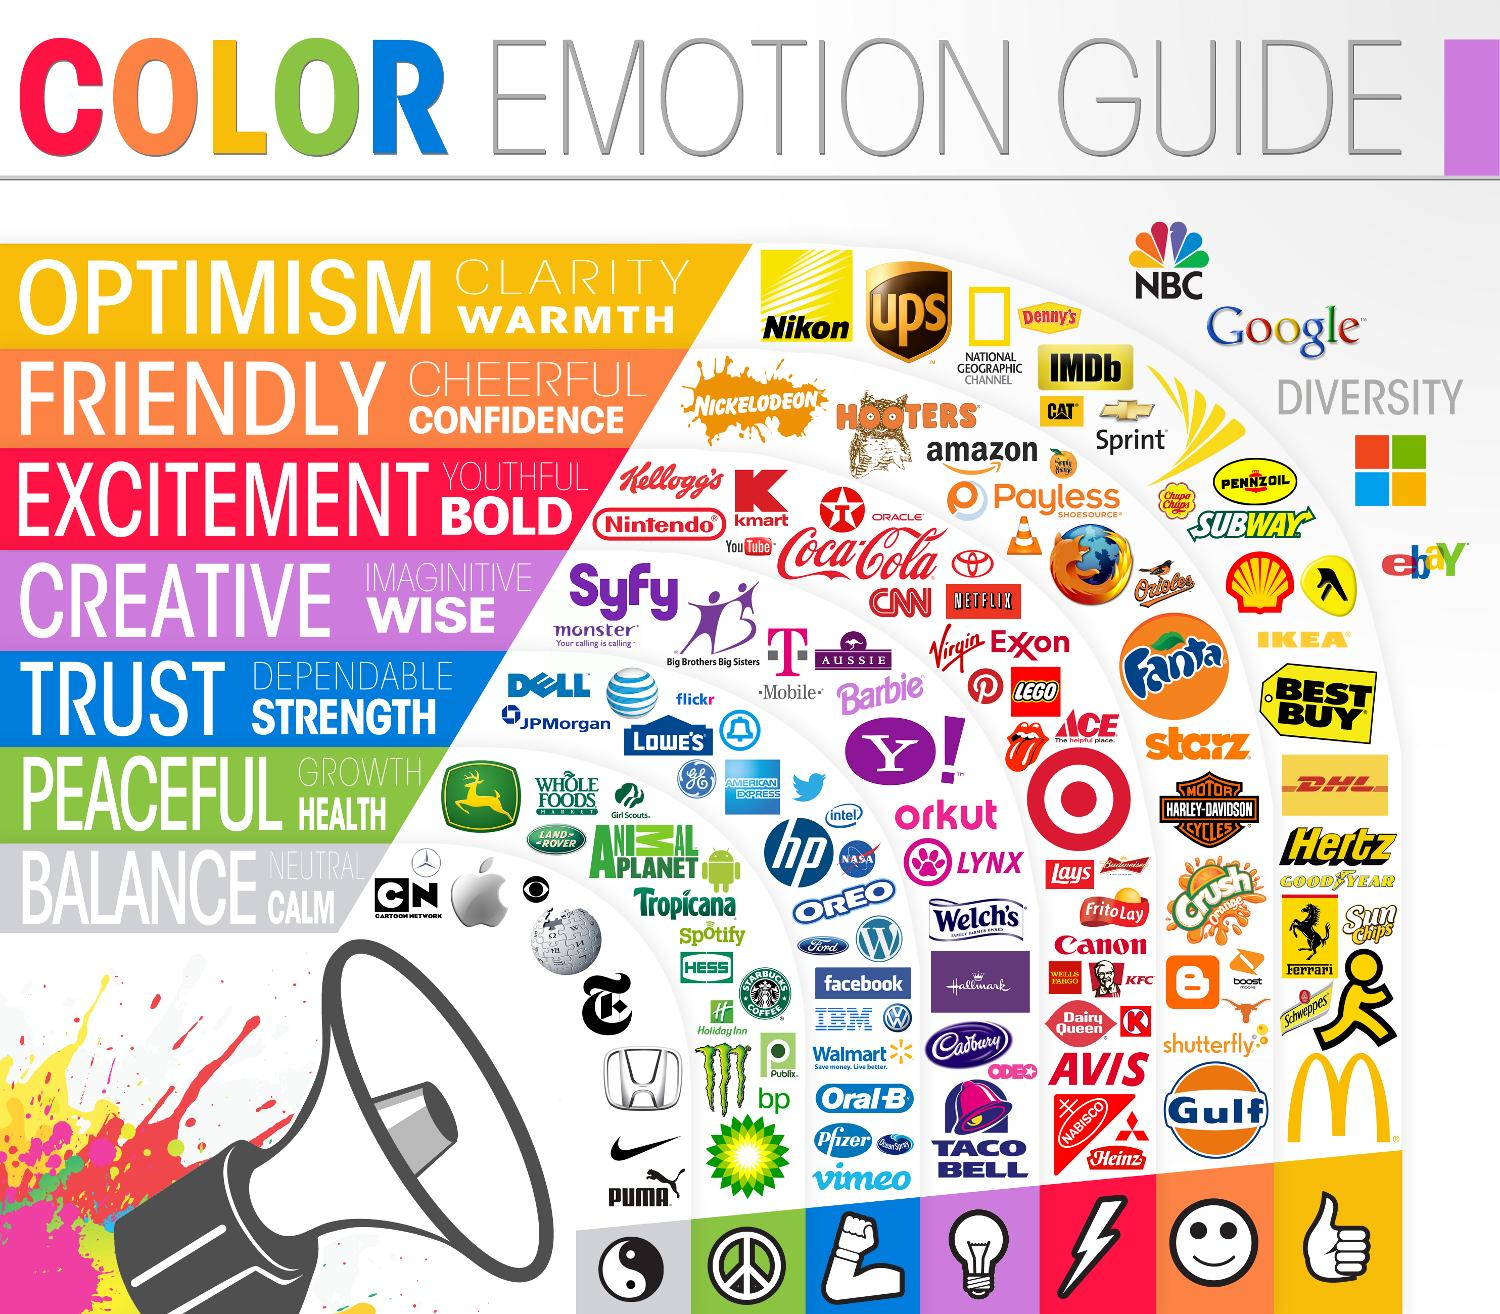
\includegraphics[scale=0.125]{color-emotion.jpg}
\caption{Overall image of how colours are generally percieved. \cite{ColorMeaning}}
\end{figure}

Colour preferences differ between genders. Women prefer soft colours and tints while men prefer bright colours and shades. \cite{ColorMeaning} Since the target group of this app is not gender specific it is important to make the app gender-neutral i.e. not to soft and feminine but at the same time not to bright. 

But all in all, the concept you are working with is key. Almost every study shows that it is greatly more important to choose a colour that shows the personality of your product than picking a stereotype colour. \cite{ColorMeaning} This app is directed towards interior design and therefore it is fitting to give the app a inspiring and creative personality. According to fig. 2.12 the color purple is the inspirational and creative color. This is very feminine but mixing it with a neutral colour like grey might just take it down a notch. 

So how does one find the best way to coordinate different colours? Research indicates that the isolation effect is very useful.

\begin{figure}[H]
\centering

\includegraphics[scale=0.5]{isolation_effect.png}
\caption{"The sign-up button stands out because it's like a red "island" in a sea of blue." \cite{ColorMeaning}}
\end{figure}

Using the isolation effect will help the user have a more efficient experience because the most important feature e.g. a "sign up here" button, stands out. \cite{ColorMeaning} (See fig. 2.13)
Research suggests that a colour scheme that consists of analogues colors and combine it with a accent complimentary color or a tertiary color is preferred among users. \cite{ColorMeaning} 
This means that the colour purple would be prefered in different shades which also will end in a greyish tone would be best percieved with a complimetary color, like yellow. A tertiary color is also prefered but as these often looks muddy this is properly not the best fit.

Last but not least; make sure that the colours are bright enough and that the contrast is sufficient since the weather can affect the UX. \cite{Graphic}

\subsubsection{Rythm, Balance and proportions}
When designing your layout it is, once again, key to keep everything simple and streamlined. 
Follow the general rules, left-to-right and top-to-bottom. Make sure the most important feature is in the top left corner where the user will look first.\cite{Graphic}

\subsubsection{Fonts}
The most popular combinations of fonts is sans serif and a serif body type. \cite{TypeComb}

Dan Mayer has created a set of guidelines to choosing a font and typeface. This consist of 5 simple rules that will make the art of choosing the right font a little easier. First thing Dan mentions is that picking a font is like picking out an outfit for the day. Appropriateness is key, although you might have some favourites that you love to use. As he says "While appropriateness isn't a sexy concept, it's the acid test that should guide our choice of font." \cite{Font}

There is a huge list of fonts to choose from. Mayer suggests that we only look at 5 key groups. 

\begin{figure}[H]
\centering
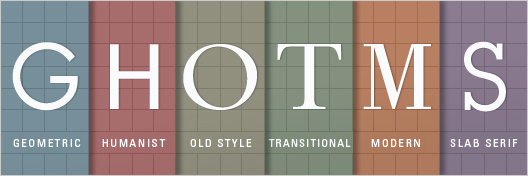
\includegraphics[scale=0.5]{type-mash.jpg}
\caption{Mayer's five groups of fonts. \cite{Font}}
\end{figure}

\begin{itemize}

\item
Geometric Sans
\\
Geometric sans is a "less is more" typeface; it is minimalistic.

"At their best, Geometric Sans are clear, objective, modern, universal; at their worst, cold, impersonal, boring. A classic Geometric Sans is like a beautifully designed airport: it's impressive, modern and useful, but we have to think twice about whether or not we'd like to live there." \cite{Font} %how do I cite this properly?

\item
Humanist Sans
\\
These Sans faces are based on hand writing. Even though some of them look clean and modern they still have a human touch. One one hand it manages to both be clear and modern but also human and empathic. One the other hand it might come across as wish-wash and and fake. \cite{Font}

\item
Old Style
\\
These are the oldest typefaces there are, hence the name. 
They are classic and traditional which can be a good or bad thing given the context. 

\item
Transitional and Modern
\\
These typefaces emerged as type designers experimented with more geometric sharp and virtuosic typefaces. 
These can seem strong, dynamic and stylish but at their worst too baroque and to stodgy. \cite{Font} 

\item
Slab Serif
\\
Slab serif is hard to generalize. It goes in many different directions and can both seem hard (Rockwell) but also friendly (Archer). As Mayer says " .. their distinctive blocky serifs function something like a pair of horn-rimmed glasses: they add a distinctive wrinkle to anything, but can easily become overly conspicuous in the wrong surroundings." \cite{Font}
\end{itemize}

Third principle - The principle of decisive contrast. When combining typefaces either go with the exact same or make a big contrast. The official name for this is Correspondence and Contrast. As the name suggests, it means that you either stay with the same typeface(correspondence) or you do something completely different(contrasting).\cite{Font}
There is no general rule to decide how to fonts go well together, they just do. But a general rule of thumb can be to choose two fonts that have one thing in common, like x-height or stroke, but are different in all other aspects. 

"A little can go a long way" is the fourth rule. In short, this teaches us that when you need something with personality only use it in a small amount. E.g. use a fun font for a headline and combine it with another more simple font for the main text. 

Mayers fifth rule is that there is no rule - the best way of finding a great fit is to try a lot of different styles. \cite{Font}

To sum up, do not overdress your text and always keep it simple. Combining a maximum of two fonts should hit the spot.\cite{TypeComb}

Be careful when choosing a font type. You cant control the devices fonts and thus try to pick an common type font.  \cite{Graphic} To make the text easy to read make sure that the contrast between text and background is present. Either black and white or a light coloured background with dark text. \cite{Graphic}